%package list
\documentclass{article}
\usepackage[top=3cm, bottom=3cm, outer=3cm, inner=3cm]{geometry}
\usepackage{multicol}
\usepackage{graphicx}
\usepackage{url}
%\usepackage{cite}
\usepackage{hyperref}
\usepackage{array}
%\usepackage{multicol}
\newcolumntype{x}[1]{>{\centering\arraybackslash\hspace{0pt}}p{#1}}
\usepackage{natbib}
\usepackage{pdfpages}
\usepackage{multirow}
\usepackage[normalem]{ulem}
\useunder{\uline}{\ul}{}
\usepackage{svg}
\usepackage{xcolor}
\usepackage{listings}
\lstdefinestyle{ascii-tree}{
    literate={├}{|}1 {─}{--}1 {└}{+}1 
  }
\lstset{basicstyle=\ttfamily,
  showstringspaces=false,
  commentstyle=\color{red},
  keywordstyle=\color{blue}
}
%\usepackage{booktabs}
\usepackage{caption}
\usepackage{subcaption}
\usepackage{float}
\usepackage{array}

\newcolumntype{M}[1]{>{\centering\arraybackslash}m{#1}}
\newcolumntype{N}{@{}m{0pt}@{}}


%%%%%%%%%%%%%%%%%%%%%%%%%%%%%%%%%%%%%%%%%%%%%%%%%%%%%%%%%%%%%%%%%%%%%%%%%%%%
%%%%%%%%%%%%%%%%%%%%%%%%%%%%%%%%%%%%%%%%%%%%%%%%%%%%%%%%%%%%%%%%%%%%%%%%%%%%
\newcommand{\itemEmail}{vmamanian@unsa.edu.pe \n rninacal@unsa.edu.pe}
\newcommand{\itemStudent}{Victor Mamani Anahua \n Rafael Nina Calizaya}
\newcommand{\itemCourse}{Fundamentos de la Programación II}
\newcommand{\itemCourseCode}{--------}
\newcommand{\itemSemester}{II}
\newcommand{\itemUniversity}{Universidad Nacional de San Agustín de Arequipa}
\newcommand{\itemFaculty}{Facultad de Ingeniería de Producción y Servicios}
\newcommand{\itemDepartment}{Departamento Académico de Ingeniería de Sistemas e Informática}
\newcommand{\itemSchool}{Escuela Profesional de Ingeniería de Sistemas}
\newcommand{\itemAcademic}{2023 - B}
\newcommand{\itemInput}{Del 15 Enero de 2024}
\newcommand{\itemOutput}{Al 16 Enero de 2024}
\newcommand{\itemPracticeNumber}{02}
\newcommand{\itemTheme}{Practica-02}
%%%%%%%%%%%%%%%%%%%%%%%%%%%%%%%%%%%%%%%%%%%%%%%%%%%%%%%%%%%%%%%%%%%%%%%%%%%%
%%%%%%%%%%%%%%%%%%%%%%%%%%%%%%%%%%%%%%%%%%%%%%%%%%%%%%%%%%%%%%%%%%%%%%%%%%%%

\usepackage[english,spanish]{babel}
\usepackage[utf8]{inputenc}
\AtBeginDocument{\selectlanguage{spanish}}
\renewcommand{\figurename}{Figura}
\renewcommand{\refname}{Referencias}
\renewcommand{\tablename}{Tabla} %esto no funciona cuando se usa babel
\AtBeginDocument{%
	\renewcommand\tablename{Tabla}
}

\usepackage{fancyhdr}
\pagestyle{fancy}
\fancyhf{}
\setlength{\headheight}{30pt}
\renewcommand{\headrulewidth}{1pt}
\renewcommand{\footrulewidth}{1pt}
\fancyhead[L]{\raisebox{-0.2\height}{
\includegraphics[width=3cm]{img/logo_episunsa.png}}}
\fancyhead[C]{\fontsize{7}{7}\selectfont	\itemUniversity \\ \itemFaculty \\ \itemDepartment \\ \itemSchool \\ \textbf{\itemCourse}}
\fancyhead[R]{\raisebox{-0.2\height}{
\includegraphics[width=1.2cm]{img/logo_abet}}}
\fancyfoot[L]{GRUPO}
\fancyfoot[C]{\itemCourse}
\fancyfoot[R]{Página \thepage}

% para el codigo fuente
\usepackage{listings}
\usepackage{color, colortbl}
\definecolor{dkgreen}{rgb}{0,0.6,0}
\definecolor{gray}{rgb}{0.5,0.5,0.5}
\definecolor{mauve}{rgb}{0.58,0,0.82}
\definecolor{codebackground}{rgb}{0.95, 0.95, 0.92}
\definecolor{tablebackground}{rgb}{0.8, 0, 0}

\lstdefinestyle{java}{frame=tb,
	language=Java,
	showstringspaces=false,
	columns=flexible,
	basicstyle={\footnotesize\ttfamily\color[RGB]{255,255,255}},
	numberstyle=\color{mygray},
	numbers=left, 
	keywordstyle=\color{myblue},
	morekeywords={String, System},
	commentstyle=\color{mygray},
	stringstyle=\color{mygreen},
	breaklines=true,
	breakatwhitespace=true,
	tabsize=2,
	backgroundcolor= \color{codebackgroundCode},
	showspaces=false,
	showtabs=false,
	showlines=false,
}

\lstset{frame=tb,
	language=bash,
	aboveskip=3mm,
	belowskip=3mm,
	showstringspaces=false,
	columns=flexible,
	basicstyle={\small\ttfamily},
	numbers=none,
	numberstyle=\tiny\color{gray},
	keywordstyle=\color{blue},
	commentstyle=\color{dkgreen},
	stringstyle=\color{mauve},
	breaklines=true,
	breakatwhitespace=true,
	tabsize=3,
	backgroundcolor= \color{codebackground},
}

\begin{document}
	
	\vspace*{10px}
	
	\begin{center}	
		\fontsize{17}{17} \textbf{ Informe de Practica \itemPracticeNumber}
	\end{center}
	\centerline{\textbf{\Large Tema: \itemTheme}}
	%\vspace*{0.5cm}	

	\begin{flushright}
		\begin{tabular}{|M{2.5cm}|N|}
			\hline 
			\rowcolor{tablebackground}
			\color{white} \textbf{Nota}  \\
			\hline 
			     \\[30pt]
			\hline 			
		\end{tabular}
	\end{flushright}	

	\begin{table}[H]
		\begin{tabular}{|x{4.7cm}|x{4.8cm}|x{4.8cm}|}
			\hline 
			\rowcolor{tablebackground}
			\color{white} \textbf{Grupo} & \color{white}\textbf{Escuela}  & \color{white}\textbf{Asignatura}   \\
			\hline 
			{\itemStudent \par \itemEmail} & \itemSchool & {\itemCourse \par Semestre: \itemSemester \par Código: \itemCourseCode}     \\
			\hline 			
		\end{tabular}
	\end{table}		
	
	\begin{table}[H]
		\begin{tabular}{|x{4.7cm}|x{4.8cm}|x{4.8cm}|}
			\hline 
			\rowcolor{tablebackground}
			\color{white}\textbf{Practica} & \color{white}\textbf{Tema}  & \color{white}\textbf{Duración}   \\
			\hline 
			\itemPracticeNumber & \itemTheme & 04 horas   \\
			\hline 
		\end{tabular}
	\end{table}
	
	\begin{table}[H]
		\begin{tabular}{|x{4.7cm}|x{4.8cm}|x{4.8cm}|}
			\hline 
			\rowcolor{tablebackground}
			\color{white}\textbf{Semestre académico} & \color{white}\textbf{Fecha de inicio}  & \color{white}\textbf{Fecha de entrega}   \\
			\hline 
			\itemAcademic & \itemInput &  \itemOutput  \\
			\hline 
		\end{tabular}
	\end{table}
	
	\section{Tarea}
	\begin{itemize}		
        \item El uso Base de Datos.
        \item Como conectar Java con la base de datos 
		\item El uso del patron de diseño Singleton para la optimizacion en la creacion de objetos.
	\end{itemize}

	\section{Equipos, materiales y temas utilizados}
	\begin{itemize}
		\item Sistema Operativo Ubuntu GNU Linux 23 lunar 64 bits Kernell 6.2.v
		\item Visual Studio Code.
		\item VIM 9.0.
		\item OpenJDK 64-Bits 19.0.7.
		\item Git 2.39.2.
		\item Cuenta en GitHub con el correo institucional.
		\item Actividades del Prac02.	
	\end{itemize}
	
	\section{URL de Repositorio Github}
	\begin{itemize}
		\item URL del Repositorio GitHub para clonar o recuperar.
		\item \url{https://github.com/VictorMA18/fp2-23b.git}
		\item URL para la prac02 en el Repositorio GitHub.
		\item \url{https://github.com/VictorMA18/fp2-23b/tree/main/Fase03/Examen-Prac02}
	\end{itemize}
	
	\section{Actividades de la Prac02}

	\subsection{Ejercicio Conectar}
	\begin{itemize}	
		\item El código Java proporciona una implementación básica de un patrón Singleton para la gestión de conexiones a una base de datos MySQL. La clase Conectar utiliza el patrón Singleton para garantizar la existencia de una única instancia de la conexión a la base de datos. La clase contiene un método estático getInstance() que devuelve la instancia única de la clase, y un método conexion() que establece la conexión a la base de datos MySQL local utilizando el controlador com.mysql.jdbc.Driver. La conexión se establece con credenciales específicas (usuario: "root", contraseña: "") y la base de datos "fp2_23b"
	\end{itemize}		
		\item Cabe mencionar que el código presenta una redundancia en la implementación del patrón Singleton con la presencia de dos campos estáticos singleton y instancia, y la ausencia de una variable de instancia real, lo cual podría llevar a confusión y no sigue estrictamente el patrón. Además, el código maneja las excepciones generales sin detallar mensajes específicos, lo cual podría dificultar la depuración en caso de errores.
	\begin{lstlisting}[language=java,caption={Las lineas de codigos del metodo creado:}][H]
		import java.sql.Connection;
		import java.sql.DriverManager;
		import java.sql.PreparedStatement;
		import java.sql.ResultSet;
		import java.sql.SQLException;
		import java.util.Properties;
		
		public class Conectar{
			private static Conectar singleton = null;
			public static synchronized Conectar getInstance(){
				if (singleton == null)
					singleton = new Conectar();
				return singleton;
			}
			private static Conectar instancia;
			Connection conectar = null;
			public Connection conexion(){
				try{
					Class.forName("com.mysql.jdbc.Driver");
					conectar = (Connection) DriverManager.getConnection("jdbc:mysql://localhost:3306/fp2_23b","root","");
					System.out.println("Conexion aceptada");
				} catch (Exception e){
					System.out.println(e);
				}
				return conectar;
			}
		}
	\end{lstlisting}
	\subsection{Ejercicio Main}
	\begin{itemize}	
		\item El código Java presenta una comparación entre la creación de instancias de la clase Conectar sin utilizar el patrón Singleton y utilizando el patrón Singleton. En la primera parte del programa, se crean tres instancias separadas de Conectar mediante el constructor, y se imprime el hashcode de cada instancia junto con la conexión a la base de datos. En la segunda parte, se utiliza el método estático getInstance() del patrón Singleton para obtener instancias de Conectar, y se imprime el hashcode junto con la conexión a la base de datos. Al usar el Singleton, se observa que las instancias tienen el mismo hashcode, indicando que se trata de la misma instancia de la clase Conectar, lo cual es característico del patrón Singleton. Este enfoque evita la creación innecesaria de múltiples instancias y garantiza una única conexión a la base de datos, promoviendo la eficiencia en la gestión de recursos.
	\end{itemize}	
	\begin{lstlisting}[language=java,caption={Las lineas de codigos del metodo creado:}][H]
		import java.sql.Connection;
		import java.sql.DriverManager;
		import java.sql.PreparedStatement;
		import java.sql.ResultSet;
		import java.sql.SQLException;
		
		public class Main {
		   public static void main(String[] args){
			   System.out.println("Sin Singleton");
			   Conectar conn1 = new Conectar();
			   System.out.println("El hashcode de conn es : " + conn1.hashCode());
			   conn1.conexion();
			   Conectar conn2 = new Conectar();
			   System.out.println("El hashcode de conn es : " + conn2.hashCode());
			   conn2.conexion();
			   Conectar conn3 = new Conectar();
			   System.out.println("El hashcode de conn es : " + conn3.hashCode());
			   conn3.conexion();
			   System.out.println("Usando Singleton");
			   Conectar conn4 = Conectar.getInstance();
			   System.out.println("El hashcode de conn es : " + conn4.hashCode());
			   conn4.conexion();
			   Conectar conn5 = Conectar.getInstance();
			   System.out.println("El hashcode de conn es : " + conn5.hashCode());
			   conn5.conexion();
			   Conectar conn6 = Conectar.getInstance();
			   System.out.println("El hashcode de conn es : " + conn6.hashCode());
			   conn6.conexion();
		   }
		}
	\end{lstlisting}
	\begin{figure}[H]
		\centering
		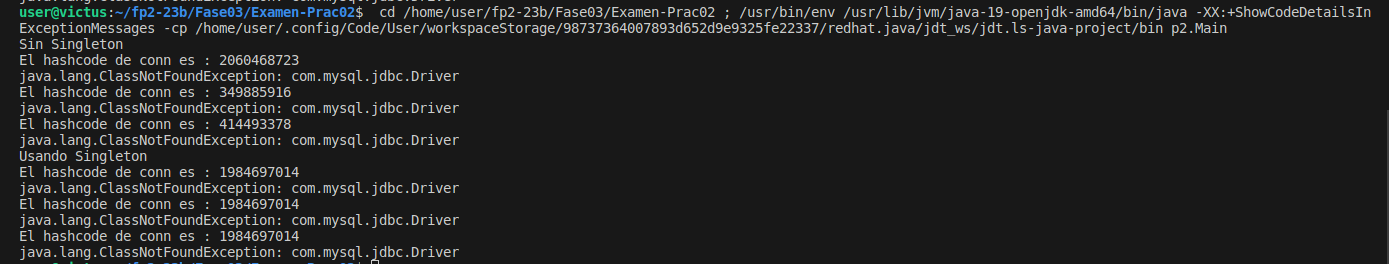
\includegraphics[width=1.0\textwidth,keepaspectratio]{img/Screen.png}
		%\includesvg{img/automata.svg}
		%\label{img:mot2}
		%\caption{Product backlog.}
	\end{figure}
	\subsection{Links Drive y los commits}
	\begin{itemize}	
		\item Aca dejaremos el link del video Drive y el commit
		\item \url{https://drive.google.com/file/d/1Qde24VzpziKqNg6vQzDnIRyhvrLZiPSU/view?usp=sharing}
	\end{itemize}	
	\begin{lstlisting}[language=bash,caption={Commit}][H]
		$ git commit -m "Agregando los archivos para la practica02"
		$ git commit -m "Imprimiendo casos donde se aplican objetos creados con y sin singleton"
	\end{lstlisting}	
	\subsection{Estructura de EXAMEN-Prac02}
	\begin{itemize}	
		\item El contenido que se entrega en esta practica02 es el siguiente:
	\end{itemize}
	\begin{lstlisting}[style=ascii-tree]
	/EXAMEN-PRAC02	
	├── Conectar.java
	├── Latex
	│   ├── img
	│   │   ├── logo_abet.png
	│   │   ├── logo_episunsa.png
	│   │   ├── logo_unsa.jpg
	│   │   └── Screen.png
	│   ├── InformePrac-02.aux
	│   ├── InformePrac-02.fdb_latexmk
	│   ├── InformePrac-02.fls
	│   ├── InformePrac-02.log
	│   ├── InformePrac-02.out
	│   ├── InformePrac-02.pdf
	│   ├── InformePrac-02.synctex.gz
	│   └── InformePrac-02.tex
	└── Main.java

	\end{lstlisting}    
	\section{\textcolor{red}{Rúbricas}}
	
	\subsection{\textcolor{red}{Entregable Informe}}
	\begin{table}[H]
		\caption{Tipo de Informe}
		\setlength{\tabcolsep}{0.5em} % for the horizontal padding
		{\renewcommand{\arraystretch}{1.5}% for the vertical padding
		\begin{tabular}{|p{3cm}|p{12cm}|}
			\hline
			\multicolumn{2}{|c|}{\textbf{\textcolor{red}{Informe}}}  \\
			\hline 
			\textbf{\textcolor{red}{Latex}} & \textcolor{blue}{El informe está en formato PDF desde Latex,  con un formato limpio (buena presentación) y facil de leer.}   \\ 
			\hline 
			
			
		\end{tabular}
	}
	\end{table}
	
	\clearpage
	
	\subsection{\textcolor{red}{Rúbrica para el contenido del Informe y demostración}}
	\begin{itemize}			
		\item El alumno debe marcar o dejar en blanco en celdas de la columna \textbf{Checklist} si cumplio con el ítem correspondiente.
		\item Si un alumno supera la fecha de entrega,  su calificación será sobre la nota mínima aprobada, siempre y cuando cumpla con todos lo items.
		\item El alumno debe autocalificarse en la columna \textbf{Grupo} de acuerdo a la siguiente tabla:
	
		\begin{table}[ht]
			\caption{Niveles de desempeño}
			\begin{center}
			\begin{tabular}{ccccc}
    			\hline
    			 & \multicolumn{4}{c}{Nivel}\\
    			\cline{1-5}
    			\textbf{Puntos} & Insatisfactorio 25\%& En Proceso 50\% & Satisfactorio 75\% & Sobresaliente 100\%\\
    			\textbf{2.0}&0.5&1.0&1.5&2.0\\
    			\textbf{4.0}&1.0&2.0&3.0&4.0\\
    		\hline
			\end{tabular}
		\end{center}
	\end{table}	
	
	\end{itemize}
	
	\begin{table}[H]
		\caption{Rúbrica para contenido del Informe y demostración}
		\setlength{\tabcolsep}{0.5em} % for the horizontal padding
		{\renewcommand{\arraystretch}{1.5}% for the vertical padding
		%\begin{center}
		\begin{tabular}{|p{2.7cm}|p{7cm}|x{1.3cm}|p{1.2cm}|p{1.5cm}|p{1.1cm}|}
			\hline
    		\multicolumn{2}{|c|}{Contenido y demostración} & Puntos & Checklist & Estudiante & Profesor\\
			\hline
			\textbf{1. GitHub} & Hay enlace URL activo del directorio para el  laboratorio hacia su repositorio GitHub con código fuente terminado y fácil de revisar. &2 &X &2 & \\ 
			\hline
			\textbf{2. Commits} &  Hay capturas de pantalla de los commits más importantes con sus explicaciones detalladas. (El profesor puede preguntar para refrendar calificación). &4 &X &2.5 & \\ 
			\hline 
			\textbf{3. Código fuente} &  Hay porciones de código fuente importantes con numeración y explicaciones detalladas de sus funciones. &2 &X &2 & \\ 
			\hline 
			\textbf{4. Ejecución} & Se incluyen ejecuciones/pruebas del código fuente  explicadas gradualmente. &2 &X &2 & \\ 
			\hline			
			\textbf{5. Pregunta} & Se responde con completitud a la pregunta formulada en la tarea.  (El profesor puede preguntar para refrendar calificación).  &2 &X &2 & \\ 
			\hline	
			\textbf{6. Fechas} & Las fechas de modificación del código fuente estan dentro de los plazos de fecha de entrega establecidos. &2 &X &2 & \\ 
			\hline 
			\textbf{7. Ortografía} & El documento no muestra errores ortográficos. &2 &X &2 & \\ 
			\hline 
			\textbf{8. Madurez} & El Informe muestra de manera general una evolución de la madurez del código fuente,  explicaciones puntuales pero precisas y un acabado impecable.   (El profesor puede preguntar para refrendar calificación).  &4 &X &2 & \\ 
			\hline
			\multicolumn{2}{|c|}{\textbf{Total}} &20 & &16.5 & \\ 
			\hline
		\end{tabular}
		%\end{center}
		%\label{tab:multicol}
		}
	\end{table}
	
\clearpage

	
%\clearpage
%\bibliographystyle{apalike}
%\bibliographystyle{IEEEtranN}
%\bibliography{bibliography}
			
\end{document}